\documentclass[letterpaper,11pt]{report}
\usepackage[T1]{fontenc}
\usepackage[utf8]{inputenc}
\usepackage{lmodern}
\usepackage{float} % for floats other than tables and graphics
\usepackage{array}
\usepackage{textcomp}
\usepackage[pdftex]{graphicx}

\floatstyle{boxed}
\newfloat{code}{h!tb}{cod}
\floatname{code}{Snippet}

\title{GAVRT Solar Patrol\\Observer's Guide}
\author{Tom Kuiper\\with help from Lilibet}

\begin{document}

\maketitle
\tableofcontents
\listoffigures
\listoftables
\listof{code}{List of Code Snippets}

\chapter{Quick Start}

\section{Quick Look}

Code snippet~\ref{cod:examdata} shows how to get a quick look at a day's data.
For more details, see section~\ref{sec:overview} (page~\pageref{sec:overview}).
\begin{code}[h!tb]
    \begin{center}
        {\footnotesize \begin{verbatim}
kuiper@kuiper:~$ cd '/usr/local/projects/SolarPatrol/apps/Reduction'
kuiper@kuiper:/usr/local/projects/SolarPatrol/apps/Reduction$ ipython --pylab
...
In [1]: run mapList.py
In [2]: sp = dbplotter.get_session_plotter(year=2019, doy=242); \
             sp.summary(save=True)
INFO:Data_Reduction.DSN.GAVRT.Mysql.plotter.DBPlotter.Session:
                                                2019/242 found 18 boresights
no usable boresights found\end{verbatim}
        }\caption{\label{cod:examdata}Quick look at the data from an observing
        session.}
    \end{center}
\end{code}



\chapter{Overview}

GAVRT Solar Patrol uses a monitor and control (M\&C) paradigm in which the 
operator manages the antenna and the receiver more or less independently using 
two separate programs.  Figure~\ref{fig:M&C} shows the GAVRT M\&C system.
\begin{figure}[h!tb]
    \begin{center}
        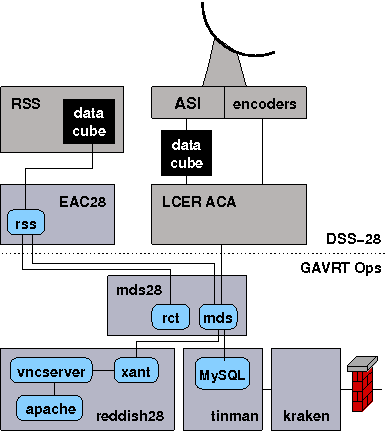
\includegraphics[width=2.7in]{DSS28-netmap.png}
        \caption{\label{fig:M&C}The GAVRT M\&C system is distributed over
            the Lewis Center in Apple Valley (control center) and DSS-28
            at Goldstone (antenna and receiver).}
    \end{center}
\end{figure}
The operator has two graphical user interfaces (GUIs) provided by the program 
{\ttfamily rss} which manages the Receiver Subsystem, and the program 
{\ttfamily xant} which mainly manages the antenna but also interacts with 
{\ttfamily rss} to get readings from the voltage-to-frequency converters 
for antenna calibration.

There is available a software package which can ``wrap'' the elements of this
system, along with other subsystems such as the digital signal processors,
into one system managed by a central server which knows the state of the
signals at each subsystem from where the signal enters the antenna to the
backend subsystems which record the data \cite{kuiper:2019}.  This may be 
implemented at a future date.

\section{Antenna}

Figure~\ref{fig:xant} shows the {\ttfamily xant} GUI which is used to monitor
and control the antenna.
\begin{figure}[h!tb]
    \begin{center}
        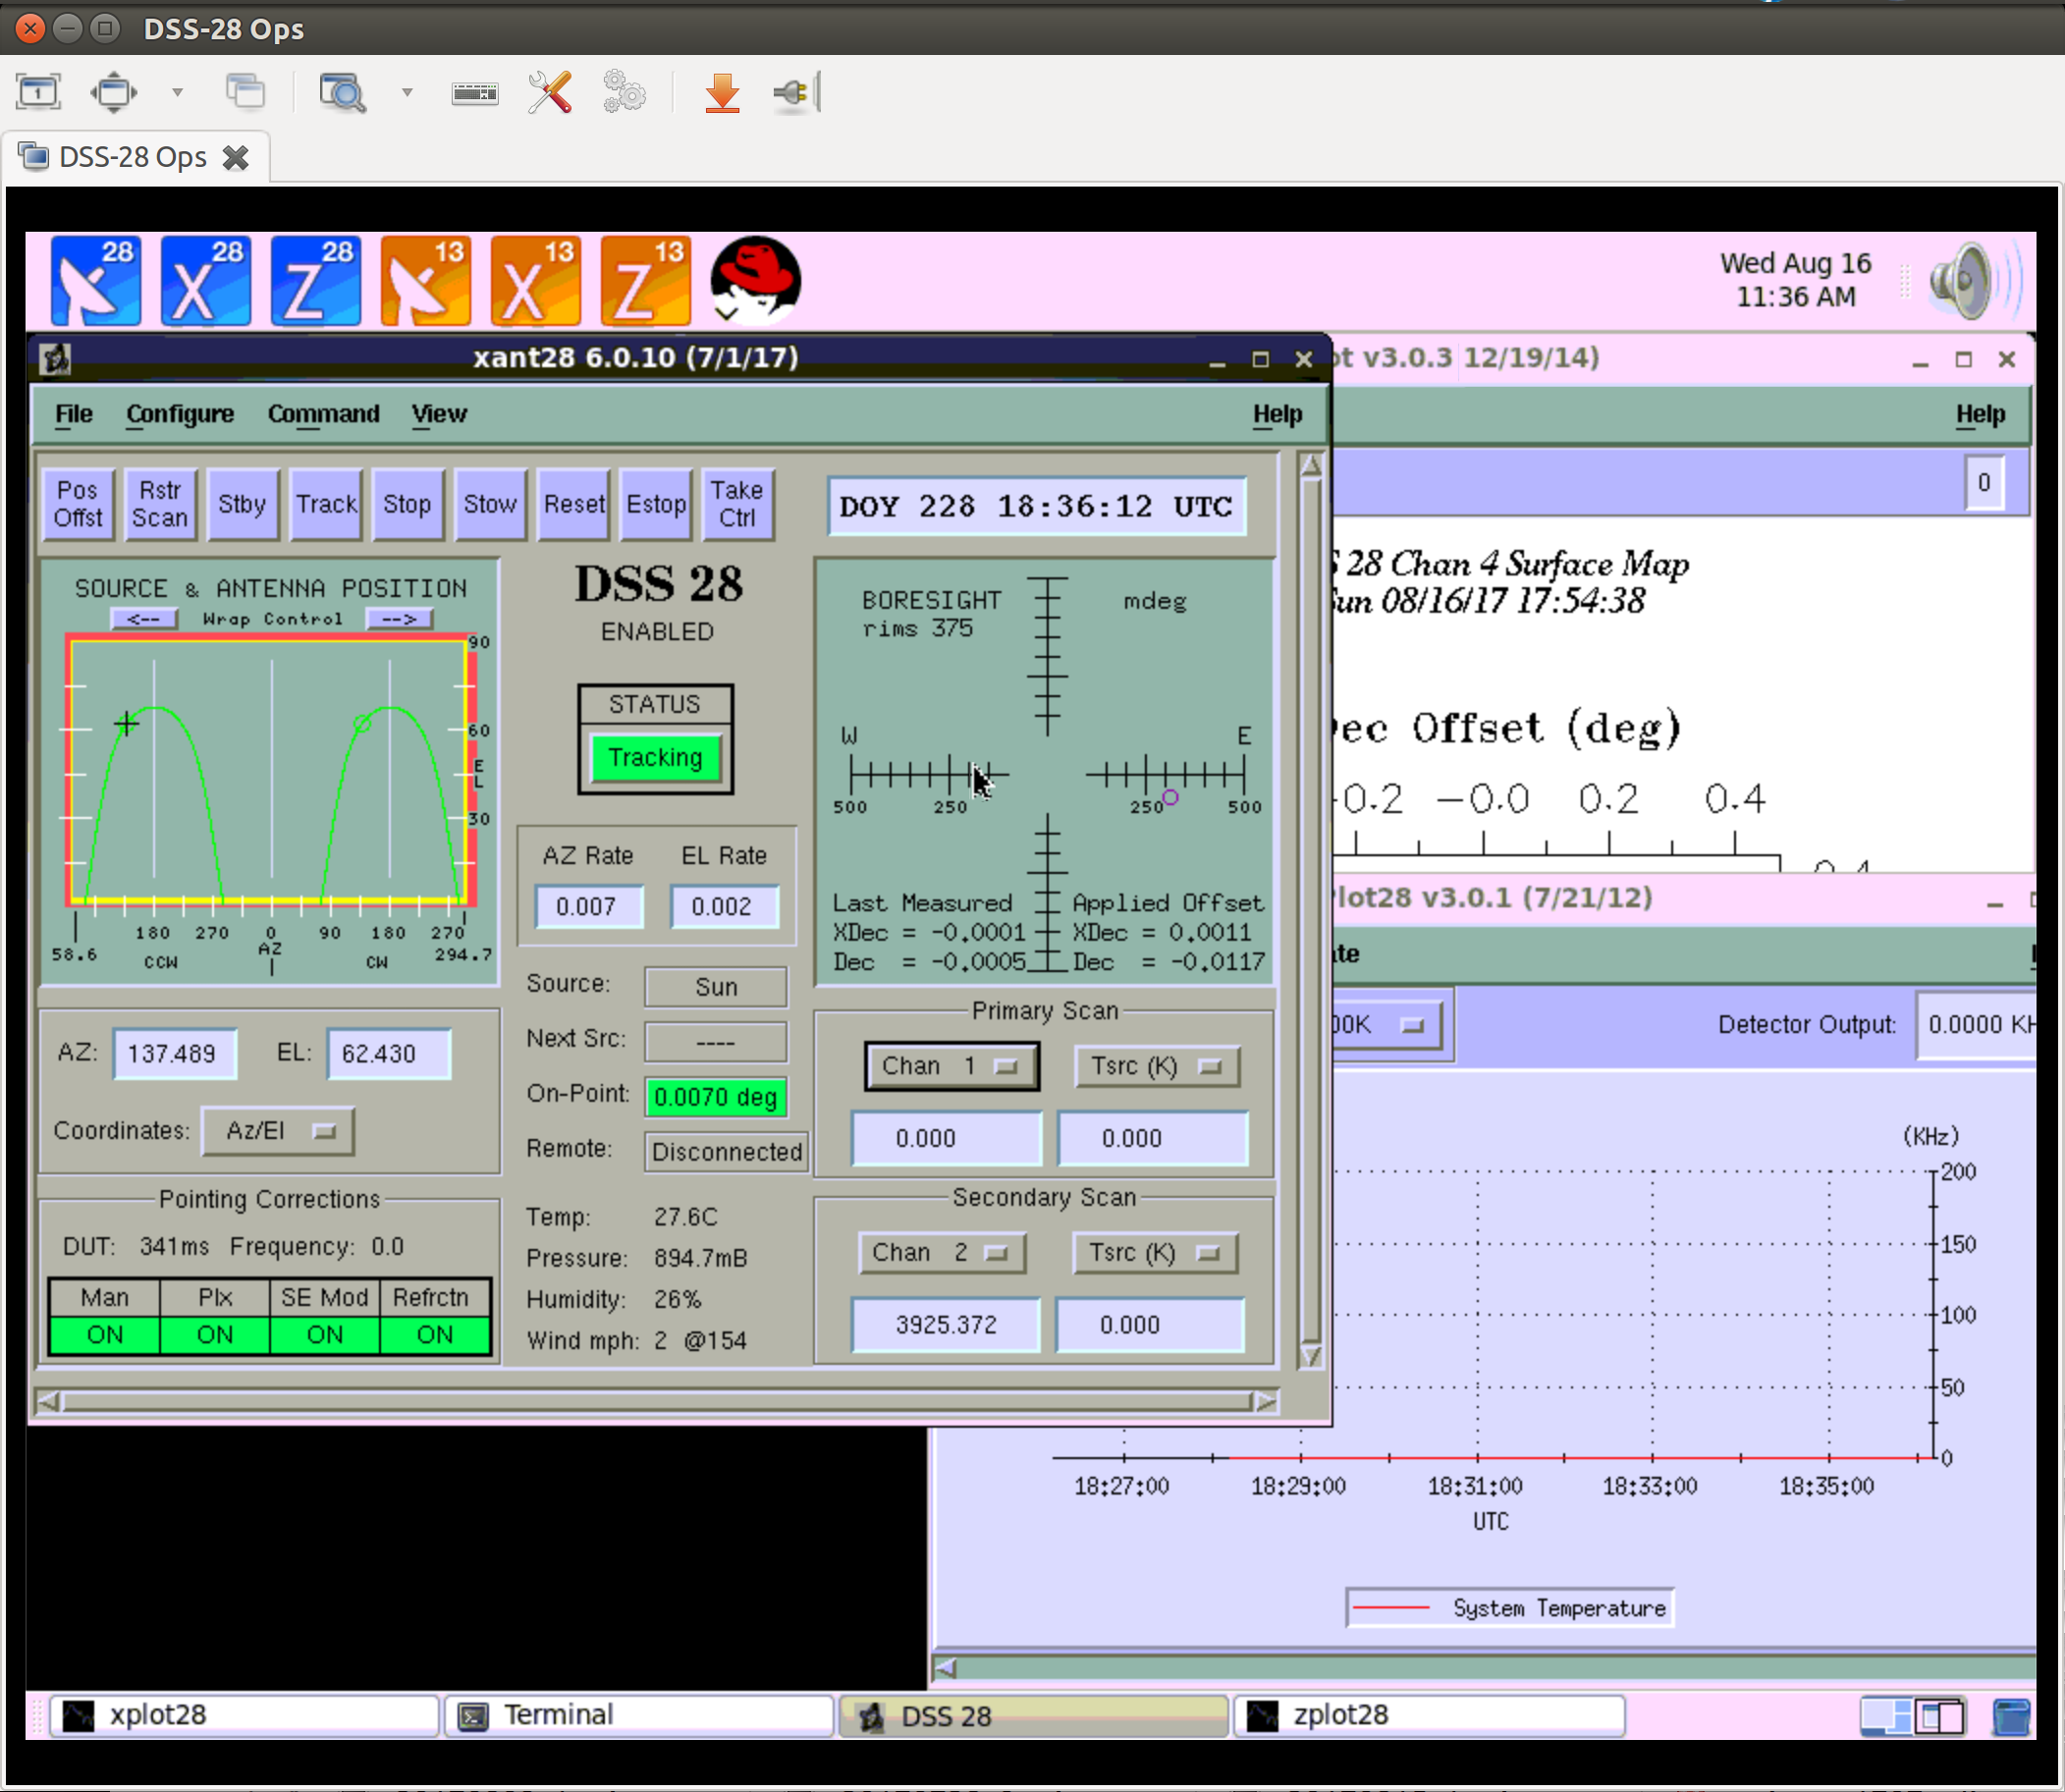
\includegraphics[width=4.5in]{DSS-28_Ops_168.png}
        \caption{\label{fig:xant}GUI for antenna M\&C.}
    \end{center}
\end{figure}
Partially hidden is the display of program {\ttfamily xplot} which is a
stripchart showing the system temperature T$_{\mbox{sys}}$ as a function of time
in one or two selected channels. Behind that is the display of program 
{\ttfamily xmap} which shows a color contour map of the source. Program 
{\ttfamily xraster}, not shown, shows a 3D image of the source.

\section{Receiver}

Figure~\ref{fig:rss} shows the {\ttfamily rss} GUI which is used to monitor
and control the receiver.
\begin{figure}[h!tb]
    \begin{center}
        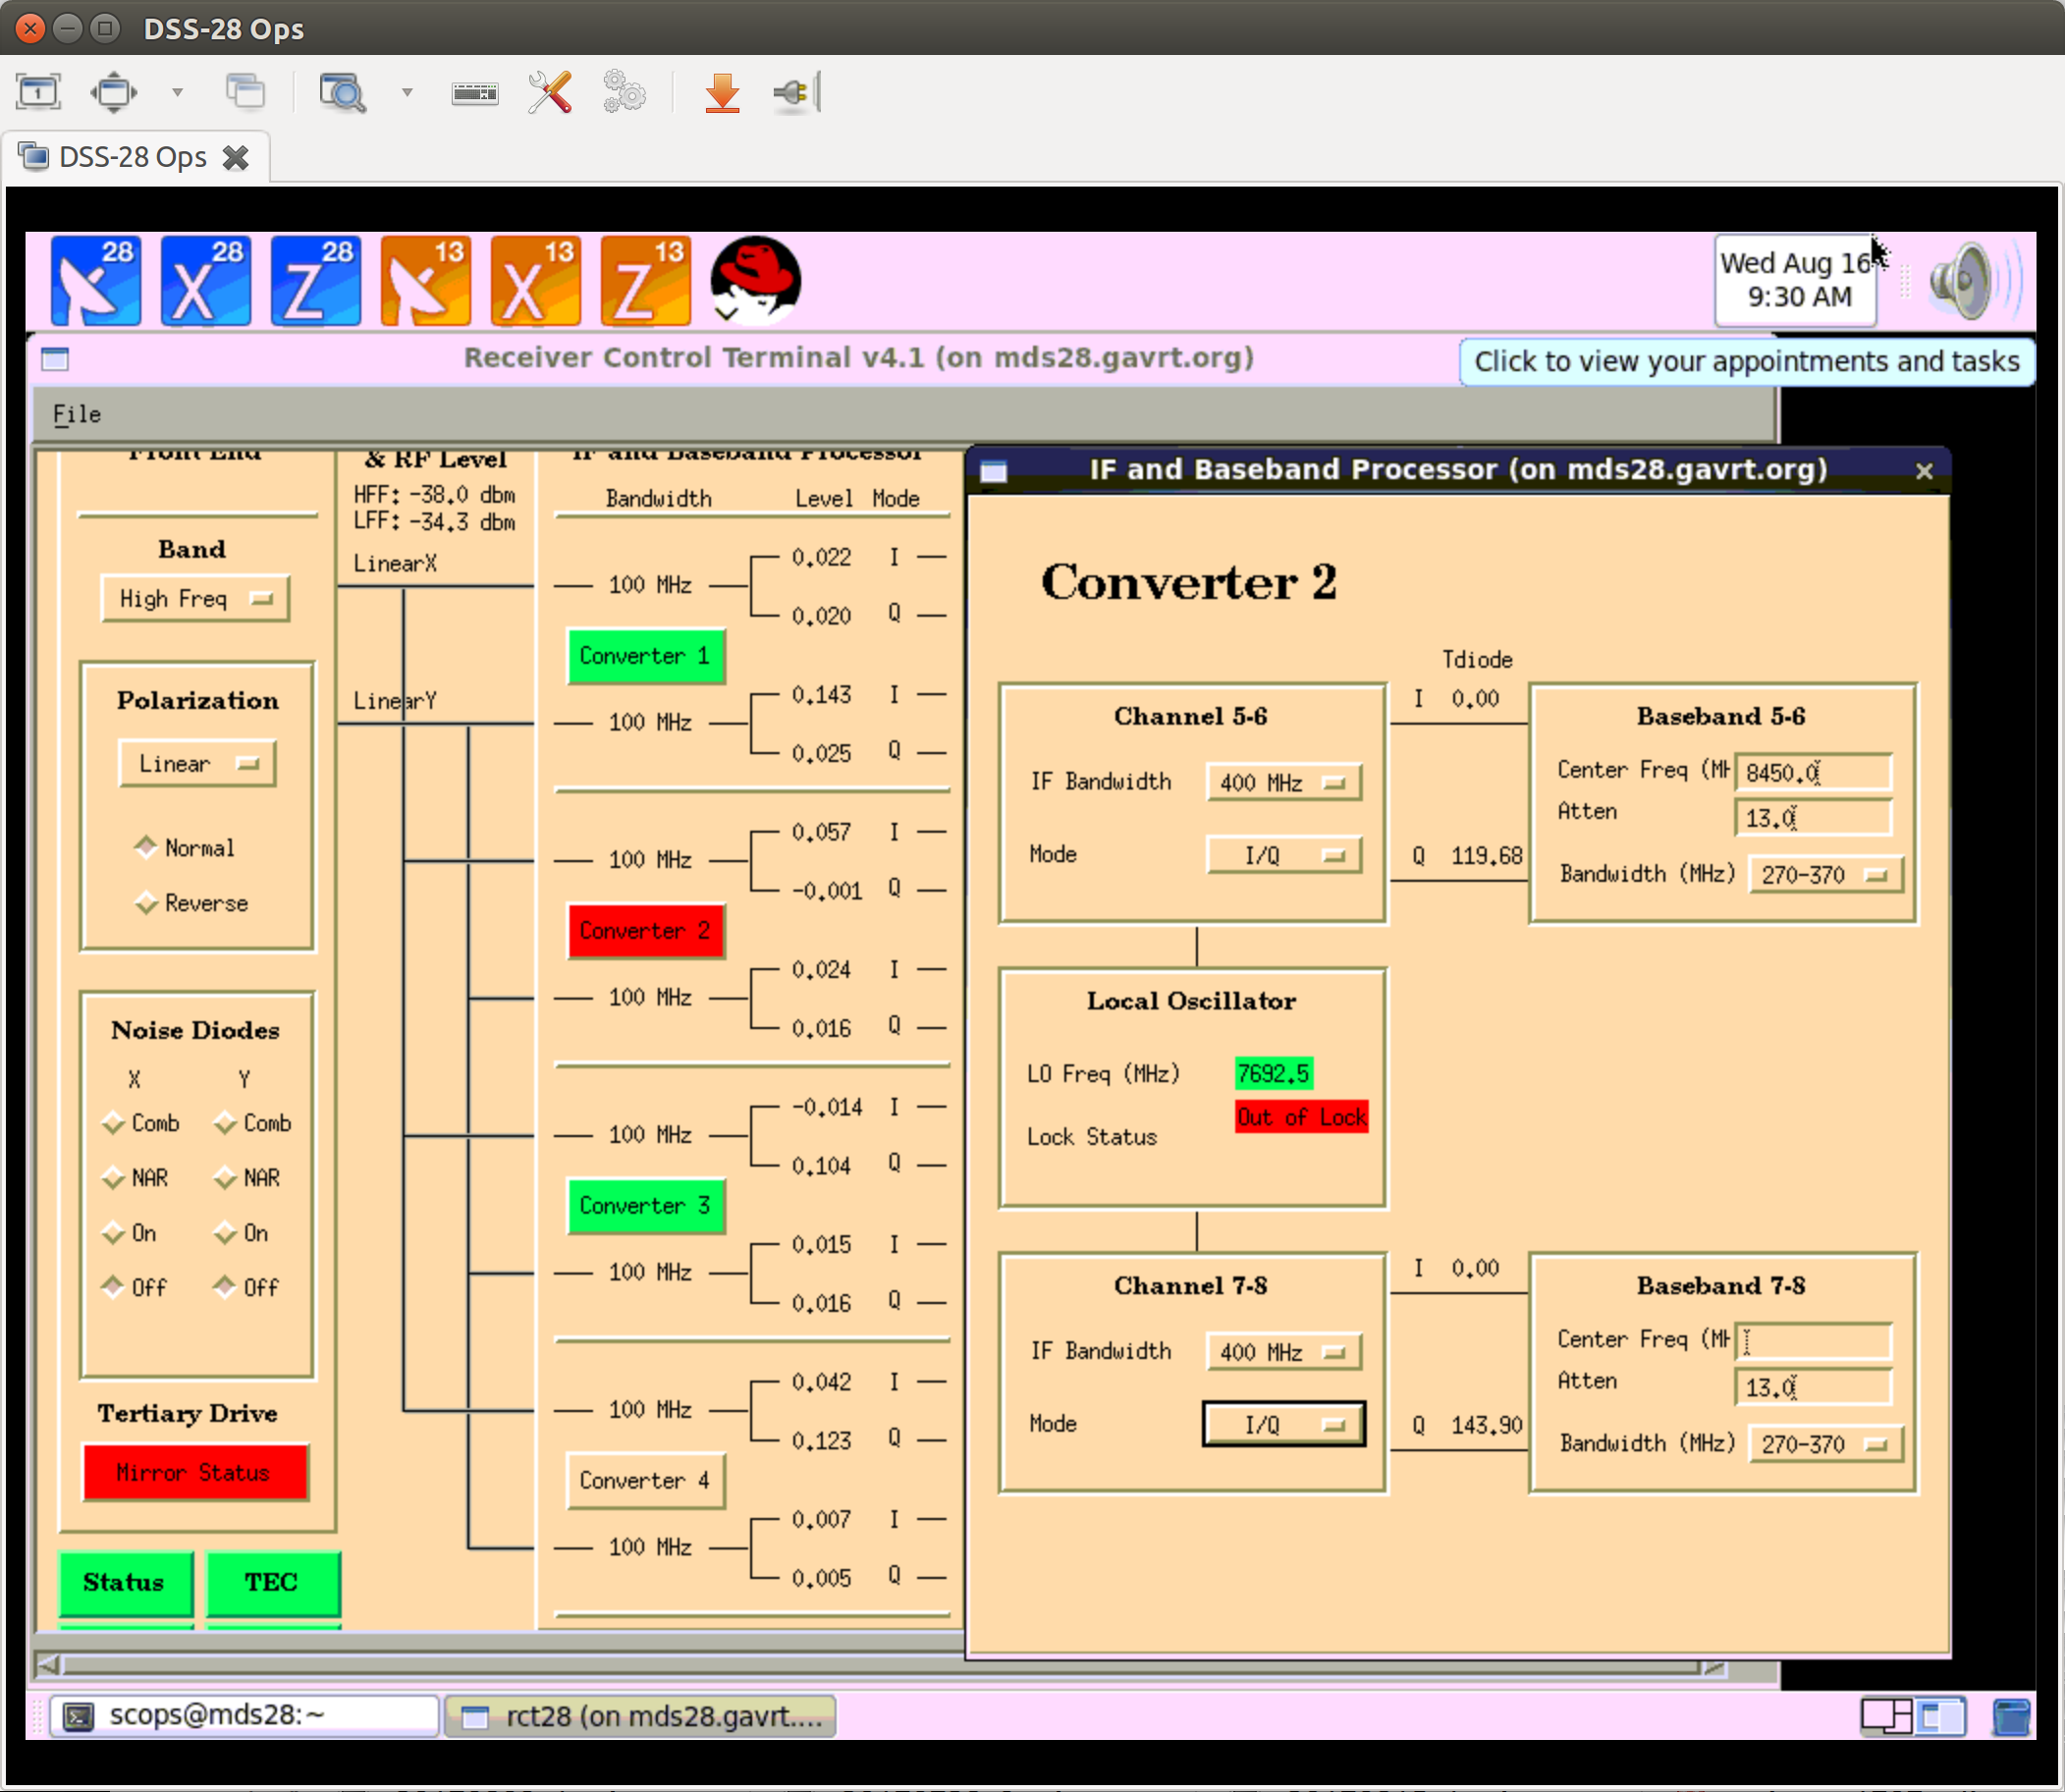
\includegraphics[width=4.5in]{DSS-28_Ops_162.png}
        \caption{\label{fig:rss}GUI for receiver M\&C.}
    \end{center}
\end{figure}
The panel labeled ``Converter 2'' is a pop-up window used to configure
one of the four down-converters.

Schematics of the DSS-28 receiver are shown in Appendix~\ref{sec:dss28rx}.
Summarizing, the receiver has two RF inputs accepting the orthogonal linear
outputs of the front end.  The signal can optionally be combined in a
quadrature hybrid to form two circular polarization. Each pair of signals 
(E-plane and H-plane, or LCP and RCP) is split by a power divider and one
copy of each is sent to one of four down-converter blocks, numbered 1-4.
The polarized inputs are referred to as ``a'' and ``b''. Each signal
(of which there are now eight copies) are down-converted to baseband in
a complex mixer which has in-phase and quadrature-phase outputs. The
outputs are usually, but not necessarily, converted to lower and upper
sidebands, giving a total of sixteen ``channels''. This is summarized
in Table~\ref{tab:chnames}
\begin{table}[h!tb]
    \begin{center}
        \caption{\label{tab:chnames}Converter and Channel Names}
        \begin{tabular}{|c|c|c|c|}
            \hline
            RF Pol. &  Down.Conv & Sideband & Channel \\
            \hline
            X/RCP   &  1a        & U        & 1 \\
                    &            & L        & 2 \\
            Y/LCP   &  1b        & U        & 3 \\
                    &            & L        & 4 \\
            \hline
            ...     &   ...      & ...      & ... \\
            \hline
            X/RCP   &  4a        & U        & 13 \\
                    &            & L        & 14 \\
            Y/LCP   &  4b        & U        & 15 \\
                    &            & L        & 16 \\
            \hline
        \end{tabular}
    \end{center}
\end{table}


\section{Software}

The software uses the object-oriented programming features of 
Python\footnote{It is possible to use Python as a procedural language such as
BASIC, C, or FORTRAN with normal functions.  The plotting package supports this 
in a 
Matlab{\textregistered}-like fashion.  With other packages or advanced
{\ttfamily matplotlib} features it becomes a challenge.}
\begin{flushright}
\framebox{\parbox{4.5in}{
\noindent {\bfseries Background} In object-oriented programming (OOP), a 
{\itshape class}
is source code for a general object, such as ``car''.  Real objects,
such as ``Tesla'', are made by creating an {\itshape instance} of a
class, called an {\itshape object}.  A class, and therefore an object,
has ``attributes'' (things with associated values, like {\ttfamily name})
and ``methods'' (functions that do things, like {\ttfamily close()}).
These are appended by name to its object name. For example
{\ttfamily datetime.strftime({\itshape format})} formats the value of
{\ttfamily datetime} according to {\itshape format}.
A  {\itshape subclass} is derived from a parent class and has all the
attributes and methods of that class, plus additional attributes and methods
of its own.}}
\end{flushright}

\noindent The class which opens and interacts with the database is {\ttfamily DSS28db}.
The class {\ttfamily DBPlotter} is a subclass of {\ttfamily DSS28db} which
adds plotting methods. The class {\ttfamily DBPlotter} is described in
Appendix~\ref{sec:dbplotter}.

All the data from a specified year and day-of-year are contained in a
class called {\ttfamily Session}.  A session object is created by specifying
the data, as in Snippet~\ref{cod:session}.
\begin{code}[h!tb]
    \begin{center}
        {\footnotesize \begin{verbatim}
from Data_Reduction.DSN.GAVRT.Mysql.dss28db import Session
session = Session(2019, 88)\end{verbatim}
        }\caption{\label{cod:session}Creating a {\ttfamily Session} object.}
    \end{center}
\end{code}
\noindent The session has an attribute called {\ttfamily maps}, which are
numbered ({\itshape e.g.} {\ttfamily session.maps[130]}).  Maps are objects of the
{\ttfamily Map} class, which is described in Appendix~\ref{sec:map}.
The subclass {\ttfamily SessionPlotter} adds plotting methods to
class {\ttfamily Session}.

\chapter{Observing Sessions}

\section{Establish a Session}

The preferred method is to start a remote desktop client with the VNC protocol.
It is also possible to download and execute a client-side Java script to run
VNC in a browser but this invites incompatibility headaches between your browser
and your version of Java.

The first step is to call GAVRT Ops at 1(760)946-5414 ext. 270 to enable remote
access to the server {\tt reddish28.gavrt.org}.

\subsection{VNC Viewer}

This will vary from desktop to destop ({\it e.g.} Gnome, Unity, KDE, etc.) but
the basic idea is to search for a remote desktop client (under "Network" if a
category is requested).  The protocol for the connection will be VNC.
The remote host and display is {\tt reddish28.gavrt.org:1}.  The password is
{\tt g4vrt4u}.

\subsection{Browser}

The browser must have Java enabled.  It may be necessary to add an exception to
allow a Java script from {\tt reddish28.gavrt.org} to run.  On a Linux system
invoke {\tt jcontrol} in a terminal window.  It will open a new window.  Under
the Security tab, look for the Exceptions site list and edit it to allow
{\tt reddish28.gavrt.org}.  Then restart the browser\footnote{In truth, I could
not get this to work for either Google Chrome or Iceweasel (=Firefox) under
Debian 7 Linux.}

\subsection{Python Connection}


\subsubsection{Receiver Configurations}

To get the current receiver configuration check the database plotter object's
{\ttfamily receiver} attribute as shown in Snippet~\ref{cod:rxcfg}
\begin{code}[h!tb]
    \begin{center}
        {\scriptsize \begin{verbatim}
In [1]: from Data_Reduction.DSN.GAVRT.Mysql.dss28db import DSS28db
In [2]: source_db = DSS28db(name='gavrt_sources')
In [3]: dbplotter.receiver
Out[3]: {'if_bw': { 2: 400.0,  4: 400.0,  6: 400.0,  8: 400.0,
                   10: 400.0, 12: 400.0, 14: 400.0, 16: 400.0},
         'if_mode': { 2: 'ul',  4: 'ul',  6: 'ul', 8:  'ul',
                     10: 'ul', 12: 'ul', 14: 'ul', 16: 'ul'},
         'pol': { 2: 'linx',  4: 'liny',  6: 'linx',  8: 'liny',
                 10: 'linx', 12: 'liny', 14: 'linx', 16: 'liny'},
         'sky_freq': { 2: 8450.0,  4: 8450.0,  6: 8450.0,  8: 8450.0,
                      10: 8450.0, 12: 8450.0, 14: 8450.0, 16: 8450.0},
         'utc': { 2: datetime.timedelta(0, 49625),  4: datetime.timedelta(0, 49625),
                  6: datetime.timedelta(0, 49625),  8: datetime.timedelta(0, 49625),
                 10: datetime.timedelta(0, 49625), 12: datetime.timedelta(0, 49625),
                 14: datetime.timedelta(0, 49625), 16: datetime.timedelta(0, 49625)}}\end{verbatim}
}\caption{\label{cod:rxcfg}Checking the current receiver configuration. (The
output has been reformatted to save space.)}
\end{center}
\end{code}


\chapter{Solar Observations}

\section{Receiver Configuration}

Table~\ref{tab:solar_cfg} shows the initial configuration for solar observations.
\begin{table}[h!tb]
    \begin{center}
        \caption{\label{tab:solar_cfg}Configuration Checklist for Solar Observations}
        \begin{tabular}{|l|c|c|}
\hline
Source                & Sun         &   Venus \\
\hline
{\bfseries Parameter} & \multicolumn{2}{c|}{\bfseries Value} \\
\hline
Absorber plate        & in          &    out \\
\hline
IF bandwidth          & \multicolumn{2}{c|}{100 MHz} \\
\hline
Polarization          & \multicolumn{2}{c|}{LCP, RCP} \\
\hline
Frequency priority    & 14, 2.8,  8.45,  4.9 & 14, 2.8,  8.45,  4.9 \\
\hline
Attenuator (without plate) & 20, 30, 30, 30 & 0, 13, 7, 7      \\
Attenuator (with plate)    & 10, 20, 20, 20 & 0, 3, 0, 0 \\
\hline
        \end{tabular}
    \end{center}
\end{table}
Depending on the number of working channels, frequencies should be selected in
the order shown with both polarizations.

The channels should be configured to write to the {\ttfamily tlog} table.

A checklist, shown in Table~\ref{tab:checklist} should be filled out for every source change.
\begin{table}[h!tb]
    \begin{center}\label{tab:checklist}
        \caption{Checklist for Each Source}
        \begin{tabular}{|l|c|c|c|c|c|c|c|c|}
\hline
Channel               & 2   &  4  &  6  &  8  & 10  & 12  & 14  & 16 \\
\hline
Polarization          & RCP & LCP & RCP & LCP & RCP & LCP & RCP & LCP \\
\hline
{\ttfamily t}log (on) &     &     &     &     &     &     &     &     \\
\hline
Frequency (GHz)       & \multicolumn{2}{c|}{} & \multicolumn{2}{c|}{} & \multicolumn{2}{c|}{} & \multicolumn{2}{c|}{} \\
\hline
Attenuation (dB)      & \multicolumn{2}{c|}{} & \multicolumn{2}{c|}{} & \multicolumn{2}{c|}{} & \multicolumn{2}{c|}{} \\
\hline
Plate (in/out)        & \multicolumn{8}{c|}{ } \\
\hline
        \end{tabular}
    \end{center}
\end{table}

\section{Checking Progress}

A {\ttfamily SessionPlotter} object let's us see what maps and boresights have
been done. Code snippet~\ref{cod:progress} shows how.
\begin{code}[h!tb]
    \begin{center}
        {\scriptsize \begin{verbatim}
In [1]: from Data_Reduction.DSN.GAVRT.Mysql.plotter import DBPlotter
In [2]: dbplotter = DBPlotter()
In [3]: sp = dbplotter.get_session_plotter(year=2019, doy=242)
In [4]: sp.summary(save=True)
In [5]: sp.maps.keys()
Out[5]: [200, 199]
In [6]: sp.boresights.keys()
Out[6]: [35201, 35202, 35203, 35204, 35205, 35206, 35207, 35208, 35209, 35210,
         35211, 35212, 35213, 35214, 35215, 35216, 35217, 35218]
In [7]: sp.maps[199].get_active_channels()
Out[7]: array([2, 4])
In [8]: sp.maps[200].get_active_channels()
Out[8]: array([2, 4])
In [9]: sp.boresights[35215].channels
Out[9]: array([2, 4])\end{verbatim}
        }\caption{\label{cod:progress}Checking progress during an observation.}
    \end{center}
\end{code}
Step [3] is slow because it searches the database for all the boresight and map 
data for that day.

Step [3] should be repeated as needed to refresh the data. {\ttfamily maps}
and {\ttfamily boresights} are those present when step~[3] is done.
{\ttfamily get\_active\_channels()} reports on the channels present in the
{\ttfamily tlog} table.  We cannot calibrate maps if there are no boresights
using the same channels.



\chapter{Data Reduction}\label{ch:datared}

All the examples here use iPython with the {\ttfamily --pylab} module.

\section{Databases}

The server has these databases: {\ttfamily dss28\_eac} is the default database.
It is described at {\ttfamily http://gsc.lewiscenter.org/data\_info/dss28\_eac.php}.
There is a database for spectrometer data called {\ttfamily dss28\_spec}.
It is described at {\ttfamily http://gsc.lewiscenter.org/data\_info/dss28\_spec.php}.
Radio source information is kept in {\ttfamily gavrt\_sources}.  It does not
have a web page describing it.

The source database can be accessed as shown in Snippet~\ref{cod:sourcedb}.
\begin{code}[h!tb]
    \begin{center}
        {\footnotesize \begin{verbatim}
In [1]: from Data_Reduction.DSN.GAVRT.Mysql.dss28db import DSS28db
In [2]: source_db = DSS28db(name='gavrt_sources')
In [3]: source_db.get_public_tables()
Out[3]: (('catalog',), ('class',), ('source',))
In [4]: source_db.get_data_index()
Out[4]: 
{'catalog': (('catalog_id', 'int(11)', 'NO', 'PRI', None, 'auto_increment'),
             ('name', 'varchar(32)', 'NO', '', None, '')),
'class': (('class_id', 'int(11)', 'NO', 'PRI', None, 'auto_increment'),
          ('name', 'varchar(32)', 'NO', '', None, ''),
          ('description', 'varchar(128)', 'YES', '', None, '')),
'source': (('source_id', 'int(11)', 'NO', 'PRI', None, 'auto_increment'),
           ('name', 'varchar(16)', 'NO', '', None, ''),
           ('RA', 'float', 'NO', '', None, ''),
           ('Dec', 'float', 'NO', '', None, ''),
           ('size_dec', 'int(11)', 'NO', '', None, ''),
           ('size_xdec', 'int(11)', 'NO', '', None, ''),
           ('catalog_id', 'int(11)', 'NO', '', None, ''),
           ('class_id', 'int(11)', 'NO', '', None, ''),
           ('reference', 'varchar(8)', 'NO', '', None, ''),sec:overview
           ('aka', 'varchar(16)', 'YES', '', None, ''))}\end{verbatim}
        }\caption{\label{cod:sourcedb}Querying {\ttfamily gavrt\_sources} for
        its tables.}
    \end{center}
\end{code}
This database can then be searched for calibration sources that fit a specific
set of requirements, such as sky position and flux density.

\subsection{Establish a Connection for Data Reduction}

Snippet~\ref{cod:opensession} shows how create a session for data reduction 
using the GAVRT MySQL database.
\begin{code}[h!tb]
    \begin{center}
{\small \begin{verbatim}
In [1]: from Data_Reduction.DSN.GAVRT.Mysql.plotter import DBPlotter
In [2]: dbplotter = DBPlotter()
...
In [6]: dbplotter.close()
\end{verbatim}
    }\caption{\label{cod:opensession}Opening and closing a data reduction 
    session using the GAVRT MySQL database.}
\end{center}
\end{code}
The {\ttfamily DBPlotter} inherits all the attributes and methods of the
{\ttfamily DSS28db} class and adds plotting using {\ttfamily matplotlib}.


\section{Public Tables}

Appendix~\ref{ch:dbtables} (page~\pageref{ch:dbtables}) gives the details of
the database tables.  If the manual isn't handy, code snippet~\ref{cod:dbtables}
shows how to ask the database for the tables.
\begin{code}[h!tb]
    \begin{center}
        {\scriptsize \begin{verbatim}
In [9]: dbplotter.get_public_tables()
Out[9]: (('angles',),       ('chan_cfg',),     ('conv_cfg',),   ('fiber_cfg',),
         ('five_point',),   ('pointing_cfg',), ('raster',),     ('raster_cfg',),
         ('rf_cfg',),       ('rss_cfg',),      ('xpwr_cfg',),   ('xscan',),
         ('zplot',),        ('zplot_cfg',))\end{verbatim}
        }\caption{\label{cod:dbtables}Example of querying a database for its
        tables.}
    \end{center}
\end{code}
To find out more about a table, get a list of its columns. Snippet~\ref{ch:datared}
shows an example.
\begin{code}[h!tb]
    \begin{center}
        {\scriptsize \begin{verbatim}
In [19]: dbplotter.get_columns('tlog')
Out[19]: (('tlog_id',    'int(11)',       'NO', 'PRI', None, 'auto_increment'),
          ('rss_cfg_id', 'int(11)',       'NO', '',    None, ''),
          ('year',       'int(4)',        'NO', '',    None, ''),
          ('doy',        'int(3)',        'NO', '',    None, ''),
          ('utc',        'time',          'NO', '',    None, ''),
          ('epoch',      'decimal(16,6)', 'NO', '',    None, ''),
          ('chan',       'int(2)',        'NO', '',    None, ''),
          ('top',        'decimal(7,4)',  'NO', '',    None, ''),
          ('integ',      'decimal(5,4)',  'NO', '',    None, ''),
          ('az',         'decimal(7,4)',  'NO', '',    None, ''),
          ('el',         'decimal(6,4)',  'NO', '',    None, ''),
          ('diode',      'tinyint(1)',    'NO', '',    None, ''),
          ('level',      'decimal(3,1)',  'NO', '',    None, ''),
          ('cryo',       'decimal(6,3)',  'NO', '',    None, ''))\end{verbatim}
        }\caption{\label{cod:tlogcols}List of columns in the {\ttfamily tlog}
        table.}
    \end{center}
\end{code}



\section{Data Analysis}

The strategy here is to give the user the full power of Python without contraint
imposed by a program with programmer defined options.  Once the basic Python
concepts have been learned this is by far the most comfortable way to work with
the data.

\subsection{Get an Overview of the Observations}\label{sec:overview}

A {\ttfamily DBPlotter} object is a {\ttfamily DSS28db} object with plotting
capability.  Code snippet~\ref{cod:progress} (page~\pageref{cod:progress})
shows how to get the maps and boresights in a table.  It produces two
files in the session directory (code snippet~\ref{cod:sesdir}),
\begin{code}[h!tb]
    \begin{center}
        {\scriptsize \begin{verbatim}
In [3]: sp.session_dir
Out[3]: '/usr/local/projects/SolarPatrol/Observations/dss28/2019/242/'
In [7]: import os
In [8]: os.listdir(sp.session_dir)
Out[8]: ['boresight-35214.png', 'boresight-35215.png', 'boresight-35216.png',  
         'boresight-35217.png', 'maps.txt',            'xscans.txt',         
         'map0199.png',         'map0200.png']
\end{verbatim}
        }\caption{\label{cod:sesdir}Getting the session directory.}
    \end{center}
\end{code}
which list the boresights and the maps. The boresights and maps are also
shown graphically, one figure for each boresight scan and map. These are 
uncalibrated VFC counts. For the maps, each figure has all the channels for that
map.

\subsection{Time Series}

The {\ttfamily tlog} table has VFC counts as a function of time, as well as
antenna angles and other variables. Code snippet~\ref{cod:tlogcols} shows
the columns of the {\ttfamily tlog} table.  The advantage of class
{\ttfamily DBPlotter} over its superclass {\ttfamily DSS28db} is that you
plot any column of the table as a time series.  Code snippet~\ref{cod:plTsys}
shows an example of that.
\begin{code}[h!tb]
    \begin{center}
        {\scriptsize \begin{verbatim}
In [20]: from DatesTimes import UnixTime_to_MPL
In [25]: Tsys_data = {2: dbplotter.get_Tsys(2, 1567198299.1872621, 
                                               1567198456.2302589),
                      4: dbplotter.get_Tsys(4, 1567198299.1872621,
                                               1567198456.2302589)}
In [26]: plot_date(UnixTime_to_MPL(Tsys_data[2]['epoch']), Tsys_data[2]['top'], '-',
                   label="Ch. 2")
In [27]: plot_date(UnixTime_to_MPL(Tsys_data[4]['epoch']), Tsys_data[4]['top'], '-',
                   label="Ch. 4")
            \end{verbatim}
        }\caption{\label{cod:plTsys}Plotting $T_{op}$ as a function of time.}
    \end{center}
\end{code}


\subsection{Boresights}

Code snippet~\ref{cod:inspect-bs} shows how to inspect boresight data.
\begin{code}[h!tb]
    \begin{center}
        {\footnotesize \begin{verbatim}
In [1]: from Data_Reduction.DSN.GAVRT.Mysql.plotter import DBPlotter
In [2]: dbplotter = DBPlotter()
In [3]: boresight_data = dbplotter.extract_boresight_data(2019,87)
In [4]: boresight_data.keys()
Out[4]: ['utc',       'el',     'rx',        'xpwr_cfg_id', 'chan',
'source',    'epoch',  'xscan_id',  'source_id',   'tsrc',
'az',        'axis']

In [7]: len(boresight_data['utc'])
Out[7]: 32
In [8]: boresight_data['rx'][0].keys()
Out[8]: ['sky_freq', 'utc', 'pol', 'if_bw', 'if_mode']

In [17]: boresight_data['source']
Out[17]: ['J1800+7828']\end{verbatim}
        }\caption{\label{cod:inspect-bs}Example to code to inspect boresight
        data}
    \end{center}
\end{code}
Getting boresight data (step [3]) takes a very long time because it involves 
look-up in 
many tables managed by the local host, so involves a lot of Internet traffic. 
Certainly time to have coffee, if not lunch. 

\subsection{Maps}

There is a quick way to get a session plotter without having to remember the
class and import path.  It's shown in code snippet~\ref{cod:startsession}.
\begin{code}[h!tb]
    \begin{center}
        {\scriptsize \begin{verbatim}
kuiper@kuiper:~$ cd '/usr/local/projects/SolarPatrol/apps/Reduction'
kuiper@kuiper:/usr/local/projects/SolarPatrol/apps/Reduction$ ipython --pylab
...
In [1]: run mapList.py
Suggestions::

* To set up a session:
sp = dbplotter.get_session_plotter(year=2019, doy=98)
* To load the boresight data and report:
sp.make_bs_dir()
* To load boresight metadata only:
xpwr_data, boresights = sp.get_boresights()
* To load boresight metadata and data:
bs_data, channels = sp.get_boresight_data() 
* To reduce boresights and maps and put results in session directory:
session_summary(sp)

To do everything at once::
sp = dbplotter.get_session_plotter(year=2019, doy=98); session_summary(sp, save=True)

Don't forget:
dbplotter.close()
when finished

In [2]: sp = dbplotter.get_session_plotter(year=2019, doy=162); sp.summary(save=True)
no usable boresights found
            \end{verbatim}
        }\caption{\label{cod:startsession}Program {\ttfamily mapList} can be used
        to get a session summary.}
    \end{center}
\end{code}
\noindent The {\ttfamily save} argument will put summary plots and text
in a directory {\small \ttfamily Observations/dss28/2019/162}.

The maps for this session can be found in attribute {\ttfamily maps} which is a
{\ttfamily dict} keyed on map number.  More useful for analysis are map plotters
which are a subclass of the maps.  Snippet~\ref{cod:mapplotters} shows how to use
them.
\begin{code}[h!tb]
    \begin{center}
{\scriptsize \begin{verbatim}
    In [5]: mpl = sp.get_map_plotters()
    In [6]: mpl.keys()
    Out[6]: [193, 194, 195, 196, 197, 198]
    In [7]: mpl193 = mpl[193]
    In [8]: mapdata = mpl193.maps_from_tlogs()
    In [9]: centered = mpl[193].center_map()
    In [10]: mpl193.contours(2)
    In [13]: from pylab import *
    In [14]: show()
    In [15]: mpl193.contours(4); show()
    In [16]: sp.show_images()\end{verbatim}
        }\caption{\label{cod:mapplotters}Producing map images.}
    \end{center}
\end{code}
A map as displayed on the operator's console by program {\ttfamily xant} is
stored in the database in the table {\ttfamily raster}. Rasters are defined
by positions that are offset in cross-elevation and elevation from the 
source position and by the VFC counts from one receiver channel. The parameters
for a raster are in table {\ttfamily raster\_cfg}.

Because the map data in {\ttfamily raster} are for only one channels, we need
to get the data for other channels from the {\ttfamily tlog} table.
In fact, we don't use the data in {\ttfamily raster} at all but use the
raster to define the start and end time.  We then get the map data from table
{\ttfamily tlog} between those to times.  That happens in step [8] above.
B.t.w., step [7] is not necessary.  Step [8] could just as well have been
{\ttfamily mpl[193].maps\_from\_tlogs()}. However, you can't
{\ttfamily Tab}-complete a {\ttfamily dict} element to get attributes and
methods.

The {\ttfamily tlog} table does not contain position offsets.  However, it does
have azimuth, elevation, and time.  With suitable coordinate conversions,
position offsets from the source can be calculated.  That is what
{\ttfamily center\_map()} [step 9] does.  {\ttfamily center\_map()} also calls 
method {\ttfamily regrid()} which interpolates the data onto a regular grid 
using a specified step size or the default from table {\ttfamily raster\_cfg}.
Then the maps can be plotted (steps [10] and [15]) for all channels.

The result of step [8] can be used for manipulating the maps. 
Snippet~\ref{cod:mapdata} shows the raw map data.
\begin{code}[h!tb]
    \begin{center}
{\scriptsize \begin{verbatim}
    In [20]: mapdata = sp.maps[199].maps_from_tlogs()
    In [21]: mapdata.keys()
    Out[21]: ['elevation', 'UNIXtime', 'pol',        'MPL_datenum', 'RA',
    'azimuth',   'freq',     'VFC_counts', 'declination']
    In [22]: mapdata['freq']
    Out[22]: {2: array([ 3100.]), 4: array([ 3100.])}
    In [25]: mapdata['VFC_counts'].keys()
    Out[25]: [2, 4]\end{verbatim}
        }\caption{\label{cod:mapdata}Data returned from {\ttfamily maps\_from\_tlogs()}.}
    \end{center}
\end{code}
These data are stored in an attribute called {\ttfamily map\_data}.
Centering the map provides additional data, shown in 
snippet~\ref{cod:centered}.
\begin{code}[h!tb]
    \begin{center}
        {\scriptsize \begin{verbatim}
In [28]: centered = sp.maps[199].center_map()
In [32]: sp.maps[199].map_data.keys()
Out[32]: ['elevation',  'UNIXtime', 'pol',  'MPL_datenum', 'dec_offset',
          'RA',         'azimuth',  'freq', 'VFC_counts',  'xdec_offset',
          'declination']\end{verbatim}
        }\caption{\label{cod:centered}Centering the map produces position
        offsets.}
    \end{center}
\end{code}
So thus we have a map for each active channel.

\appendix

\chapter{Database Tables}\label{ch:dbtables}

The databases used by Solar Patrol are on a MySQL
server\footnote{\ttfamily http://gsc.lewiscenter.org/data\_info/dss28\_eac.php}
at the Lewis Center.

The server has these three databases:
\begin{center}
    \begin{tabular}{l|l}
        \hline
        Name                        & Data \\
        \hline
        {\ttfamily dss28\_eac}      &  all the data from all the observations \\
        {\ttfamily dss28\_spec}     &  data from the digital spectrometers \\
        {\ttfamily gavrt\_sources}  &  radio sources used for observation and calibration \\
        \hline
    \end{tabular}
\end{center}

The main databases used by Solar Patrol are {\ttfamily dss28\_eac}, which
contains all the data about telecope and receiver operations, and
{\ttfamily gavrt\_sources}. Figure~\ref{fig:dbases}
\begin{figure}[h!tb]
    \begin{center}
        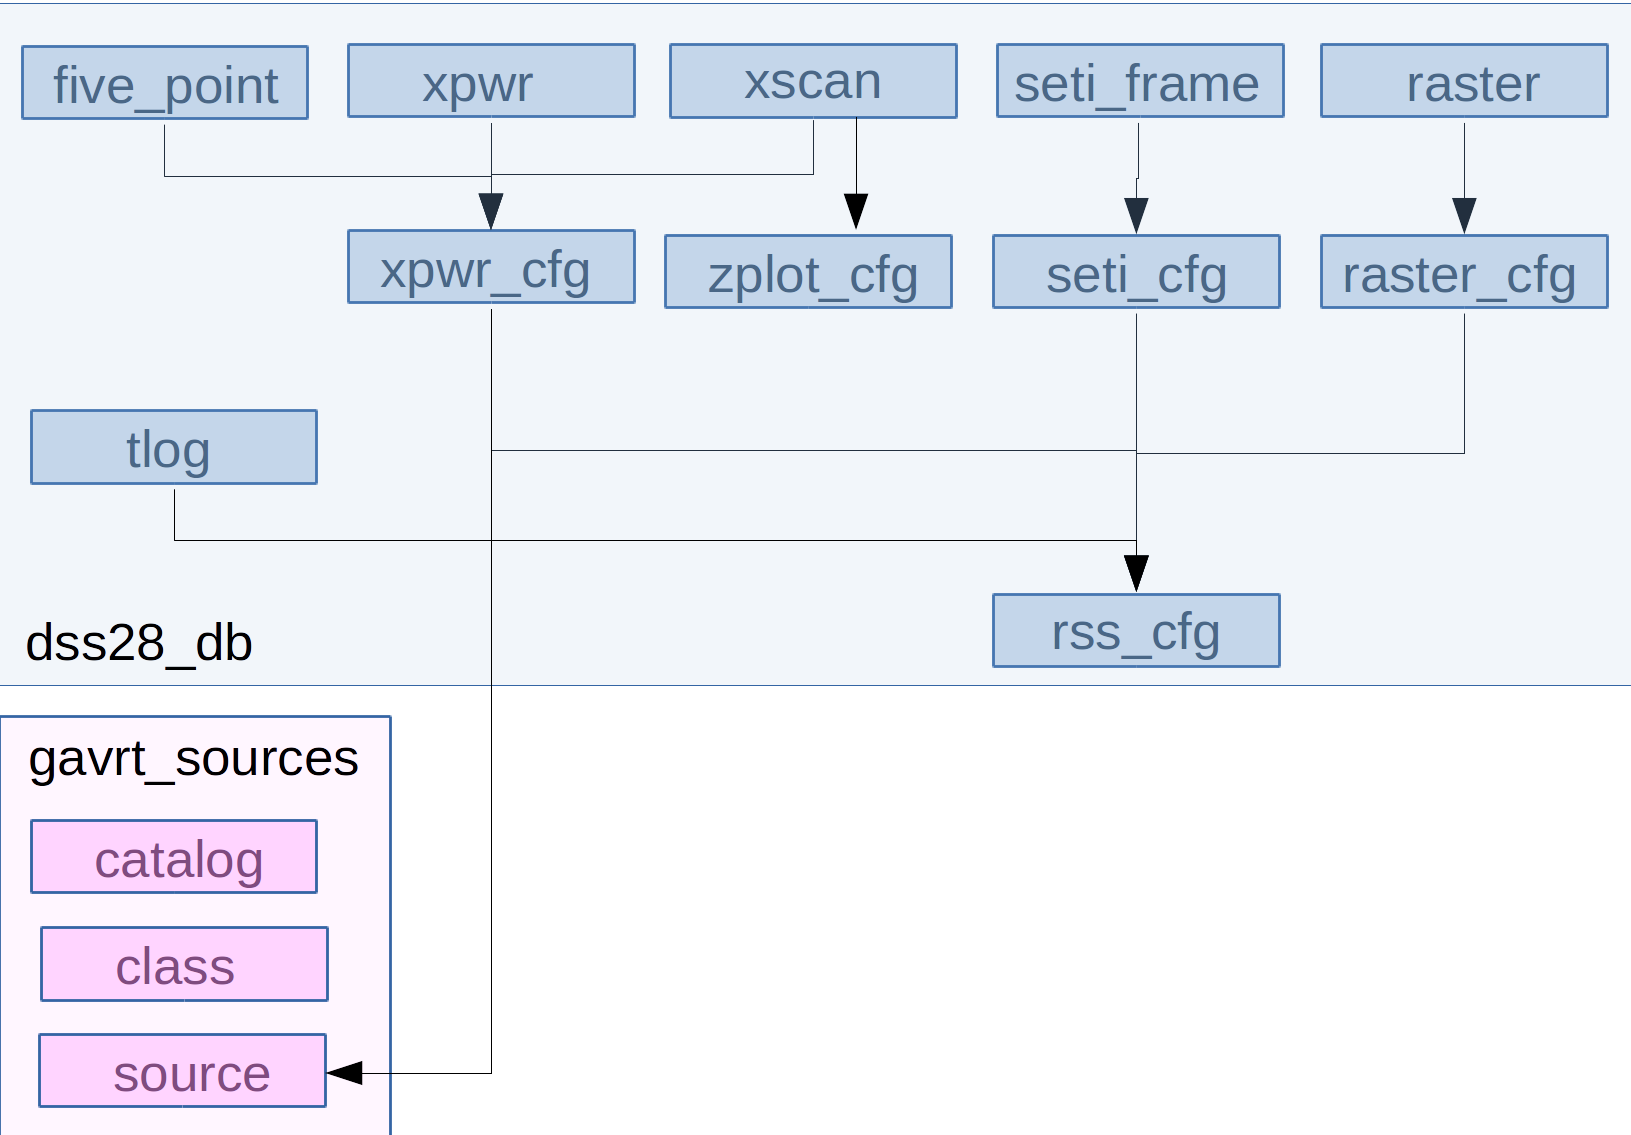
\includegraphics[width=4in]{db_relations.png}
        \caption{\label{fig:dbases}The relations between the tables used by
            Solar Patrol.}
    \end{center}
\end{figure}
The diagram can help structure queries.


Database 'gavrt\_sources' has these tables:
\begin{center}
    \begin{tabular}{l|p{4in}}
        \hline
        Name                & Contents \\
        \hline
        {\ttfamily catalog} & \\
        {\ttfamily class}   & \\
        {\ttfamily source}  & source\_id, catalog\_id, class\_id, name, RA, Dec, 
        size\_dec, size\_xdec, reference, aka \\
        \hline
    \end{tabular}
\end{center}

Database {\ttfamily dss28\_eac} has the tables shown in Table~\ref{tab:eac-cols}.
\begin{table}[h!tb]
    \caption{\label{tab:eac-cols}Columns in the tables of database 
        {\ttfamily dss28\_eac}.}
\begin{center}
    \begin{tabular}{l|p{4in}}
        \hline
        Name                       & Contents \\
        \hline
        {\ttfamily angles}         & angles\_id, year, doy, utc, epoch, az, el, 
                                     status \\
        {\ttfamily chan\_cfg}      & chan\_cfg\_id, year, doy, utc, epoch, chan, 
                                     center\_freq, tdiode \\
        {\ttfamily conv\_cfg}      & conv\_cfg\_id, year, doy, utc, epoch, 
                                     converter, mode\_a, ifbw\_a, bbbw\_a, 
                                     atten\_a, mode\_b, ifbw\_b, bbbw\_b, 
                                     atten\_b, lock\_status \\
        {\ttfamily fiber\_cfg}     & fiber\_cfg\_id, year, doy, utc, epoch, 
                                     fiber, chan \\
        {\ttfamily five\_point}    & five\_point\_id, xpwr\_cfg\_id, year, doy,
                                     utc, epoch, source\_id, chan, tsrc, azel,
                                     ha, dec, xdec\_off, dec\_off \\
        {\ttfamily pointing\_cfg}  & pointing\_cfg\_id, year, doy, utc, epoch, 
                                     man, plx, semod, refrctn, delut, model \\
        {\ttfamily raster}         & raster\_id,  raster\_cfg\_id, year, doy, utc,
                                     epoch, xdecoff, decoff, ha, dec, tsrc \\
        {\ttfamily raster\_cfg}    & raster\_cfg\_id, rss\_cfg\_id, year, doy, 
                                     utc, source\_id, chan, freq, rate, step \\
        {\ttfamily rf\_cfg}        & rf\_cfg\_id, year, doy, utc, epoch, feed,
                                     diode\_x, diode\_y, pol, transfer \\
        {\ttfamily rss\_cfg}       & rss\_cfg\_id, year, doy, utc, epoch, chan,
                                     sky\_freq, feed, pol, nd, if\_mode, if\_bw,
                                     bb\_bw, fiber\_chan\\
        {\ttfamily seti\_cfg}      & seti\_cfg\_id, rss\_cfg\_id, year, doy,
                                     utc, epoch, frame\_name, chan, freq, 
                                     school\_id, comment\\
        {\ttfamily seti\_frame}    & frame\_id, seti\_cfg\_id, year, doy, utc,
                                     epoch, glong, glat, long\_err, lat\_err \\
        {\ttfamily tlog}           & tlog\_id, rss\_cfg\_id, year, doy, utc,
                                     epoch, chan, top, integ, ax, el, diode, 
                                     level, cryo \\
        {\ttfamily weather}        & weather\_id, datetime, pressure, temp, 
                                     humidity, wind\_speed, wind\_dir \\
        {\ttfamily xpwr}           & xpwr\_id, xpwr\_cfg\_id, year, doy, utc, 
                                     epoch, tsys, az, el, ha, dec, offset \\
        {\ttfamily xpwr\_cfg}      & xpwr\_cfg\_id, rss\_cfg\_id, source\_id, 
                                     cal\_src\_id, year, doy, utc, epoch, axis, 
                                     chan, cal\_flux \\
        {\ttfamily xscan}          & xscan\_id, xpwr\_cfg\_id, year, doy, utc, epoch, 
                                     tsrc, stdev, bl\_stdev, az, az\_offset, el,
                                     el\_offset, ha, dec, offset, bw, corr \\
        {\ttfamily zplot}          & zplot\_id, zplot\_cfg\_id, offset, tsrc \\
        {\ttfamily zplot\_cfg}     & zplot\_cfg\_id, rss\_cfg\_id, year, doy,
                                     utc, epoch, source\_id, axis, chan \\
        \hline
    \end{tabular}
\end{center}
\end{table}
Most columns have self-explanatory names but a few need some description.
\begin{description}\itemsep0pt \parskip0pt \parsep0pt
    \item[\ttfamily cal\_src\_id] identifies the source which has a flux
        {\ttfamily cal\_flux} used the scale the data for the source
        {\ttfamily source\_id}.
\end{description}


\chapter{Flux Calibration}

The primary VLA flux
calibrators\footnote{\ttfamily https://science.nrao.edu/facilities/vla/docs/manuals/oss2013B/performance/fdscale}
are shown in Table~\ref{tab:fluxcal}.
\begin{table}[h!tb]
    \begin{center}\label{tab:fluxcal}
        \caption{Flux densities (Jy) of Standard Calibrators (January 2012)}
\begin{tabular}{|lcl|rrrrr| }
\hline       
       & &                    & \multicolumn{5}{c|}{Frequency (GHz)} \\
\cline{4-8}
\multicolumn{3}{|c|}{Source} & 1.465  & 2.565  & 4.885 & 8.435 & 14.965 \\
\hline
3C48   &=& J0137+3309         & 15.56 &  9.80 & 5.39 & 3.14 & 1.77 \\
3C138  &=& J0521+1638         &  8.71 &  6.17 & 4.02 & 2.78 & 1.89 \\
3C147  &=& J0542+4951         & 21.85 & 13.75 & 7.59 & 4.49 & 2.59 \\
\hline
3C286  &=& J1331+3030         & 14.90 & 10.03 & 7.34 & 5.09 & 3.39 \\
3C295  &=& J1411+5212         & 22.15 & 12.95 & 6.41 & 3.34 & 1.62 \\
NGC7027 &&                    &  1.62 &  3.59 & 5.38 & 5.79 & 5.62 \\
\hline
       \end{tabular}
    \end{center}
\end{table}
The source 3C286 (J1331+3030) is known to be non-variable, and has thus been 
adopted as the prime flux density calibrator source for the VLA. The adopted 
polynomial expression for the spectral flux density for 3C286 
is\footnote{\ttfamily https://science.lbo.us/facilities/vla/docs/manuals/oss/performance/fdscale}:
\begin{equation}
\log(S) = 1.2515 - 0.4605\log(f)  - 0.1715\log^2(f) + 0.0336\log^3(f)
\end{equation}
where $S$ is the flux density in Jy, and $f$ is the frequency in GHz.

The sources 3C48, 3C138, and 3C147 are all slowly variable. 
Table~\ref{tab:fluxcal2} shows the flux values four years 
later\footnote{\ttfamily https://science.nrao.edu/facilities/vla/docs/manuals/oss/performance/fdscale}.
\begin{table}[h!tb]
    \begin{center}\label{tab:fluxcal2}
        \caption{Flux densities (Jy) of Standard Calibrators (January 2016)}
        \begin{tabular}{|lcl|rrrrr| }
            \hline       
            & &                    & \multicolumn{5}{c|}{Frequency (GHz)} \\
            \cline{4-8}
\multicolumn{3}{|c|}{Source} &  1.50 &   3.00 &	6.00 & 10.00 & 15.00 \\
3C48$^*$ &=& J0137+3309      & 15.40 &   8.44 & 4.42 &  2.68 & 1.79	\\
3C138    &=& J0521+1638      & 08.25 &   5.44 & 3.39 &  2.33 & 1.72	\\
3C147    &=& J0542+4951      & 21.00 &  12.00 & 6.45 &  3.99 & 2.73	\\
\hline
3C196    &=& J0813+4813      & 13.60 &   6.98 & 3.38 &  1.91 & 1.20	\\
3C286    &=& J1331+3030      & 14.60 &   9.91 & 6.39 &  4.50 & 3.37	\\
3C295    &=& J1411+5212      & 21.20 &  11.00 & 5.06 &  2.70 & 1.60	\\
\hline      
        \end{tabular}\\
    \end{center}
    $^*$The flux density scale calibrator 3C48 has been undergoing a flare 
    since January 2018 or so
\end{table}
The polynomial expression for the spectral flux density for 3C286 in 2016 is:
\begin{equation}
\log(S) = 1.2481 - 0.4507\log(f) - 0.1798\log^2(f) + 0.0357\log^3(f).
\end{equation}




\chapter{Data Reduction Tool Documentation}


\section{Radio Astronomy Software Tools}

The repository collection ``Single Dish Rasdio Astronomy Software Tools''\footnote{\ttfamily https://sdrast.github.io/} describes the modules used to reduce Solar Patrol data. The principal Python module {\ttfamily GAVRT} in in the package {\ttfamily Data\_Reduction}\footnote{\ttfamily https://github.com/SDRAST/Data\_Reduction/}.  Figure~\ref{fig:import-map} shows how it depends on other packages in the collection.
\begin{figure}[h!tb]
	\begin{center}
		\includegraphics[width=4in]{importMap}
		\caption{\label{fig:import-map}Interdependency of packages in the collection Radio Astronomy Software Tools.}
	\end{center}
\end{figure}

\section{Package {\ttfamily Data\_Reduction}}

The base module of this package provides the base classes for the package

\subsection{Class {\ttfamily Observation}}

{\ttfamily Data\_Reduction.Observation} is the superclass which provides the data structure and methods common to all observations. Conceptually, the data structure {\ttfamily data} is a table, though it is implemented as a Python {\ttfamily dict}.  

\subsubsection{Attributes}

These are the public attributes of the class:
\begin{description}\itemsep0pt \parskip0pt \parsep0pt
	\item[aliases] [{\ttfamily list}] are {\ttfamily data} keys used to replace those in original data, in order to have a common format.
	\item[channel] [{\ttfamily Channel} instance] is a signal paths; {\itshape e.g.}, for different frequencies and polarizations.
	\item[data] [{\ttfamily dict}] are the original observation data, {\itshape e.g.}, read from file or database.
	\item[DOY] [{\ttfamily int}] is day of year of observation (1-366).
	\item[end] [{\ttfamily float}] is the UNIX time (Python {\ttfamily time.time}) at the end of the observation.
	\item[latitude] [{\ttfamily float}] is the telescope latitude, also an attribute of {\ttfamily obs}.
	\item[logger] [{\ttfamily logging.Logger} instance] is used to log program events.
	\item[longitude] [{\ttfamily float}] telescope longitude, also an attribute of {\ttfamily obs}.
	\item[name] [{\ttfamily str}] is assigned by the user, but defaults to YEAR/DOY.
	\item[numdata] [{\ttfamily int}] is number of data samples.
	\item[obs] [{\ttfamily Astronomy.DSN\_coordinates.DSS} instance] is the telescope.
	\item[session] [{\ttfamily Session} instance] is a set of observations, parent to Observation.
	\item[session\_path] [{\ttfamily str}] is the directory for the session's files.
	\item[start] [{\ttfamily float}] is UNIX time at the beginning of the observation.
	\item[year] [{\ttfamily int}] is the year at the start of the observation.
\end{description}

\subsubsection{Data Structure Keys}

The data structure must have these keys (table column names) or version (in {\ttfamily aliases} that can map into them:
\begin{description}\itemsep0pt \parskip0pt \parsep0pt
	\item[unixtime] [{\ttfamily float}] the UNIX time in seconds,
	\item[chan\_name]  [{\ttfamily str}] the channel name,
	\item[integr] [{\ttfamily float}] integration time (exposure) in seconds,
	\item[azel] [{\ttfamily (float,float)} tuple] azimuth and elevation in decimal degrees, and
	\item[power]  [{\ttfamily float}] the power level, if only a single channel ({\ttfamily i.e.} not spectra).
\end{description}
The following keys are optional, but they are reserved names:
\begin{description}\itemsep0pt \parskip0pt \parsep0pt
	\item[diode] [{\ttfamily float}] is noise diode power in K.
	\item[level] [{\ttfamily float}] is an unidentified quantity in GAVRT database ``tlog`` table.
	\item[cryotem] [{\ttfamily float}] is the cryostat temperature in K.
	\item[windspeed] [{\ttfamily float}] is the wind speed km/hr.
	\item[winddir] [{\ttfamily float}] is the wind direction, azimuth in degrees.
	\item[ambtemp] [{\ttfamily float}] is the outside air temperature in degrees C.
	\item[pressure] [{\ttfamily float)} is the atmospheric pressure in mbar.
\end{description}

\subsubsection{Data Format Alternatives}

The original data come from many different telescopes and so the software is versatile in what it accepts. Accordingly, all the names here are reserved keywords so the software will recognize and convert data as needed.

\paragraph{Time} may also be specified as either year, DOY, UTC ({\ttfamily int}, {\ttfamily int}, colon-delimited {\ttfamily str}) or a time string such as {\ttfamily 2020/06/14/14:22:21.00}. To facilitate using the {\ttfamily matplotlib} package, time is also retained in the form of {\ttfamily datenum} values.

\paragraph{Power} may take the form of {\ttfamily Top} or {\ttfamily Tsys}, or {\ttfamily vfc\_counts}.

\paragraph{Channel} may be designated with an {\ttfamily int}, as in ``IF number'', with a lookup table.

\paragraph{Coordinates} can take many different forms which are implicitly the same as {\ttfamily az, el} tuples. For example, {\ttfamily az} and {\ttfamily el} may be in separate columns.  Other possible specifications are:
\begin{description}\itemsep0pt \parskip0pt \parsep0pt
	\item[radec] [{\ttfamily (float,float)}] precessed right ascension in decimal hours and precessed declination in decimal degrees;
	\item[radec1950]  [{\ttfamily (float,float)}] mean right ascension in decimal hours and mean declination in decimal degrees at epoch of observation;
	\item[radec2000] [{\ttfamily (float,float)}] mean right ascension in decimal hours and mean declination at equinox in decimal degrees.
\end{description}
The columns of tuples may also be given as individual columns.

\subsection{Class {\ttfamily DataGetterMixin}}

This class is for getting data from a CSV file.

\subsection{Class {\ttfamily GriddingMixin}}

This is the class for all the data and methods associated with a raster scan map.  It is expected that the parent class is a subclass of ``Observation`` already by virtue of it being a superclass of subclass which inherits these methods.

\subsection{Class {\ttfamily Map(Observation, GriddingMixin)}}\label{sec:map}

General {\ttfamily Map} class without special features for GAVRT and Malargue.  Most of the methods are mixed in to avoid conflicting with subclasses.

\subsection{Class {\ttfamily Recording}}

Class for raw IF voltage data.  This is typically the contents of a data file transcribed into a standard format.  It may be the data of one {\ttfamily Observation} object, or data for multiple {\ttfamily Observation} objects, or contain part of the data for an{\ttfamily  Observation} object.

\subsection{Class {\ttfamily Session}}

This is the base class for an observing session on a given year and DOY.  A session usually refers to a telescope, date and project.  This will normally define a path to the session directory.

\subsubsection{Public Attributes}

\begin{description}\itemsep0pt \parskip0pt \parsep0pt
	\item[doy] [{\ttfamily int}] is the day of year for the session.
	\item[logger] [{\ttfamily logging.Logger}] - logging.Logger object
	\item[parent] may be a data reduction session for multiple observing sessions.
	\item[year] [{\ttfamily int}]   
	\item[doy] [{\ttfamily int}]
	\item[project] [{\ttfamily str}] 
	\item[session\_dir] [{\ttfamily str}] is the path to results from this session.
\end{description}

\subsection{Class {\ttfamily Spectrum (Observation)}}

This is a class for spectra.

\section{Module {\ttfamily GAVRT}}

The module called {\ttfamily DR} here is the base {\ttfamily Data\_Reduction} module desribed anbove.

\subsection{Class {\ttfamily Observation(DR.Observation, DR.GriddingMixin)}}

\subsection{Class {\ttfamily Map(Observation)}}

\subsubsection{Attributes}

\begin{description}\itemsep0pt \parskip0pt \parsep0pt
    \item[cfg] raster configuration
    \item[cfg\_id] entry in the raster configuration table
    \item[channels] list of channels which took {\ttfamily tlog data}
    \item[end] UNIX time at end of map
    \item[logger] logging.Logger object
    \item[map\_data] dict of data from {\ttfamily tlog} table;
    \item[name] map identifier
    \item[raster\_data] data from the raster table
    \item[regrid] computes map data onto a rectangular grid
    \item[rss\_cfg] receiver configuration
    \item[session] observing session to which this map belongs
    \item[start] UNIX time at start of map
\end{description}

\subsubsection{Methods}

\begin{description}\itemsep0pt \parskip0pt \parsep0pt
    \item[center\_map]  converts map coordinates to be relative to Sun
    \item[get\_active\_channels] returns channels which took tlog data during this map
    \item[get\_map\_config] returns a dict with the raster map configuration
    \item[get\_raster\_data] gets the data for a raster scan map used for Zplot
    \item[get\_raster\_keys] returns rasters associated with a given configuration
    \item[maps\_from\_tlogs] re-organizes tlog table data into map form
\end{description}

\subsection{Class {\ttfamily BoresightScan(Observation)}}

\subsubsection{Attributes}

This is the class for a single scan during a boresight. It inherits from 
class {\ttfamily Observation}.  It has these public attributes.
\begin{description}\itemsep0pt \parskip0pt \parsep0pt
    \item[\ttfamily axis] (str) direction of the scan.
    \item[\ttfamily cal\_flux] (float) flux of the calibrator source.
    \item[\ttfamily cal\_src] source used to set the flux scale.
    \item[\ttfamily chan] channel used for the boresight by EAC program 'xant'.
    \item[\ttfamily data] scan data ['el', 'az', 'tsys', 'epoch', 'ha', 'dec'] 
                          from 'xpwr' table
    \item[\ttfamily diode] state of the noise diode.
    \item[\ttfamily epoch] (float) UNIX time start of scan (not the time of the
                           first data point).
    \item[\ttfamily freq] (float) channel frequency in MHz.
    \item[\ttfamily IFbw] (float) IF band width in MHz.
    \item[\ttfamily IFmode] (str) IF phasing.
    \item[\ttfamily logger] (logging.Logger) object.
    \item[\ttfamily log\_data] data from 'tlog' table.
    \item[\ttfamily name] identifier string based on {\ttfamily xpwr\_cfg\_id}.
    \item[\ttfamily pol] channel polarization.
    \item[\ttfamily session] parent Session object.
    \item[\ttfamily source]  name of scanned source.
\end{description}

\subsection{Class {\ttfamily Session(DR.Session}}

\subsection{Class {\ttfamily DSS28db(mysql.BaseDB)}}

\section{module {Data\_Reduction.GAVRT.plotter}}

\subsection{Class {\ttfamily DBPlotter}}\label{sec:dbplotter}

\subsubsection{Attributes} 

Public attributes:
\begin{description}\itemsep0pt \parskip0pt \parsep0pt
    \item[logger] logging.Logger object
\end{description}

\noindent Attributes inherited from DSS28db:
\begin{description}\itemsep0pt \parskip0pt \parsep0pt
    \item[receiver] receivers which provide data
    \item[sessions] dict of sessions obtained with 'get\_session'
\end{description}

\subsubsection{Methods}

Method resolution order:
\begin{itemize}\itemsep0pt \parskip0pt \parsep0pt
    \item DBPlotter
    \item Data\_Reduction.DSN.GAVRT.Mysql.dss28db.DSS28db
    \item Data\_Reduction.DSN.GAVRT.Mysql.BaseDB
\end{itemize}


\noindent Methods defined here:
\begin{description}\itemsep0pt \parskip0pt \parsep0pt
    \item[\_\_init\_\_(self)] 
    \item[get\_session\_plotter(self, year, doy)] get IDs for an observing session
\end{description}
Methods inherited from Data\_Reduction.DSN.GAVRT.Mysql.dss28db.DSS28db:
\begin{description}\itemsep0pt \parskip0pt \parsep0pt
    \item[extract\_boresight\_data(self, year, doy)] Get the metadata for the boresights on the designated day.    
    \begin{description}\itemsep0pt \parskip0pt \parsep0pt
        \item[year] (int) year of observation
        \item[doy] (int) day of year
    \end{description}
    The boresights are extracted from table 'xscan'.  Missing 'el' data are
    obtained from table 'xpwr'.  The source, scan axis and channel are obtained
    from table 'xpwr\_cfg'.  The receiver data are obtained from table 'rss\_cfg'.
    
    Returns a dictionary like this:: \\
    \begin{tabular}{ll}
        'utc'&        list of datetpime.timedelta \\
        'epoch'&      list of float \\
        'az'&         list of float \\
        'el'&         list of value \\
        'chan'&       list of int \\
        'tsrc'&       list of float \\
        'axis'&       list of str \\
        'source'&     list of str \\
        'xpwr\_cfg\_id& list of int' \\
        'xscan\_id'&   list of int \\
        'source\_id'&  list of int \\
        'rx'&         list of dict \\
    \end{tabular} \\
    
    An 'rx' dict looks like this:: \\
    \begin{tabular}{lll}
        2& 'if\_bw' &    float \\
        & 'if\_mode' &  str \\
        & 'pol' &      str \\
        & 'sky\_freq' & float \\
        & 'utc' &      datetime.timedelta \\
        4 &  ...  & \\
        &  .... & \\
        16 & { ... } & \\
    \end{tabular} \\
    \item[get\_Tsys(chan, start, stop)] Get system temperatures from tlog\\
    \begin{tabular}{ll}
        start & (float) UNIXtime at start of selection \\
        stop & (float) UNIXtime at end of selection \\
    \end{tabular}\\
    \item[get\_receiver\_data (year, doy, time, columns)] Get the receiver 
    state at a given time.\\
    \begin{tabular}{ll}
        db & (Mysql.BaseDB) database \\
        year & (int) year of observation \\
        doy & (int) day of year \\
        time & (datetime.timedelta) UTC for the requested receiver state\\
        columns & (list of str) data items to be returned
    \end{tabular}\\
    This creates a dictionary keyed with channel number and returns a dictionary
    of the receiver configuration, keyed with specified in the columns, that was
    in effect at the given time.
    
    \paragraph{Notes} (Logic) The challenge here is to get the latest configuration 
    data for each channel at or prior to the specified time.  That channel may have 
    been consubsectiond on the same day or a prior day. The method we'll use is to find 
    the ID of last configuration change and assume that the IDs are sequential in 
    date/time.
    \item[get\_session(self, year, doy)] Get IDs for an observing session
\end{description}
Methods inherited from Data\_Reduction.DSN.GAVRT.Mysql.BaseDB:
\begin{description}\itemsep0pt \parskip0pt \parsep0pt
    \item[checkDB()] Reconnects to the database if the connection has been lost.
    \item[close()] Close a connection.
    \item[commit()] Commits the most recent database transaction.
    \item[connect()]  Make a connection to the database. Creates a cursor object.
    
    Automatically invoked when an instance is created; can be called
    again if the connection is closed but the database object persists
    \item[cursor()] Creates a database cursor object; same as BaseDB.c but this
    is better because it handles disconnected a database.
    \item[get(*args)] Executes a query of the database.\\
    \begin{tabular}{ll}
        args & query to be executed  \\
        return & record (dict) \\
    \end{tabular}
    \item[ getLastId(table)] (int) ID of the last record.\\
    \begin{tabular}{ll}
        table & (str) the name of the table \\
        return & ID (int) \\
    \end{tabular}
    \item[getLastRecord(table)] Returns the last record as a dictionary.\\
    \begin{tabular}{ll}
        table & (str) name of the table \\
        return & (dict) \\
    \end{tabular}
    \item[getRecordById(table, rec\_id] Get the record with the given ID.\\
    \begin{tabular}{ll}
        table & (str) table name \\
        id & (int) row ID \\
        return] & (dict) \\
    \end{tabular}
    \item[get\_as\_dict(*args, **kwargs)] Executes a query of the database and
    returns the result as a dict.
    
    At present, only keyword {\ttfamily asfloat: True} is recognized and 
    is the default if not given.  It will convert to float any values for 
    which it is possible.
    
    If the query returns multiple rows, each value associated with a keyword 
    will be a list. If nothing was found, an empty dictionary is returned.\\
    \begin{tabular}{ll}
        db & database connection object \\
        args & query to be executed \\
        kwargs & a dictionary with keyword arguments \\
        return & the record as a dictionary \\
    \end{tabular}
    \item[get\_columns(table)] Returns information about the columns of a table.
    \item[get\_data\_index()]
    \item[get\_public\_tables()] List the table names in the database.\\
    \begin{tabular}{ll}
        return &  tuple of tuples of str \\
    \end{tabular}
    \item[get\_rows\_by\_date(table, columns, year, doy)] Gets data from a table.\\
    \begin{tabular}{ll}
        table & (str) table name \\
        columns & (list of str) list of columns to be selected \\
        year & (int) \\
        doy &(int) day of year \\
        return & (dict of numpy arrays) keyed on column name \\
    \end{tabular}
    \item[get\_rows\_by\_time(table, columns, year, doy, utcs)] Queries a table 
    for quantities in columns at designated times.
    
    This loops over a list of UTs.  For each, it takes the first row it finds 
    matching the date and time.  So it has an effective resolution of one second.\\
    \begin{tabular}{lp{3.75in}}
        table & (str) table name \\
        columns & (list of str) list of columns to be selected \\
        year & (int) \\
        doy & (int) day of year \\
        utcs & (list of int) UNIX times (seconds since the epoch) to be 
        selected; the first occurrence is used \\
        return & dict of numpy arrays keyed on column name \\
    \end{tabular}
    \item[report\_table(table, columns)] Reports on the columns in a table.
    Response has keys: Extra, Default, Field, Key, Null, Type\\
    \begin{tabular}{ll}
        table & (str) table name \\
        columns & (list of str) list of column names \\
        return & result of query \\
    \end{tabular}
    \item[send\_query(query)] Send a MySQL query\\
    \begin{tabular}{ll}
        crsr  & cursor object for a database \\
        query & (str) MySQL query \\
        return & (str) query response
    \end{tabular}
\end{description}

\section{Module {\ttfamily Data\_Reduction.boresight\_fitter}}

\subsection{Class {\ttfamily ScanFitter}}

This provides an object to fit a scan in one direction to a baseline and a 
Gaussian.

\subsubsection{Methods}

Methods defined here:
\begin{description}\itemsep0pt \parskip0pt \parsep0pt
    \item[\ttfamily \_\_init\_\_(scan)] Initiate a scan fitter
    \item[\ttfamily fit\_gaussian(self, beam\_limit=2.5)] Extract the 
    appropriate data.
    
    For raster scans, {\ttfamily xdec}  means that the cross-declination
    stays fixed while the antenna moves up and down; {\ttfamily dec} means that
    declination stays fixed while the antenna moves left and right.
    
    The Gaussian is assumed to fit the inner $2\times${\ttfamily beam\_limit}
    (default: 2.5) beam widths of the data.  The baseline is the rest of the 
    data, although the lower baseline includes at least {\ttfamily data[:5]}
    and the upper baseline includes {\ttfamily data[-5]}.
   \end{description} 
 
\subsubsection{Attributes}

Public attributes:
\begin{description}\itemsep0pt \parskip0pt \parsep0pt
    \item[\ttfamily atten] (float) receiver channel attenuation for this scan.
    \item[\ttfamily baseline\_pars] (nparray) polynomial parameters for baseline.
    \item[\ttfamily calibrator] (Astronomy.Ephem.calibrator) calibrator source.
    \item[\ttfamily data] (nparray) VFC count.
    \item[\ttfamily ddecs] (nparray) declination offsets.
    \item[\ttfamily direction] (str) scan axis.
    \item[\ttfamily dxdecs] (nparray) cross-declination offsets.
    \item[\ttfamily logger] (logging.Logger)
    \item[\ttfamily pars] (nparray) Gaussian parameters.
\end{description}


\chapter{Receiver}\label{sec:dss28rx}

Figure~\ref{fig:rx-overview} shows an overall schematic of the DSS-28 receiver.
\begin{figure}[h!tb]
    \begin{center}
        % trim arguments: left bottom right top
        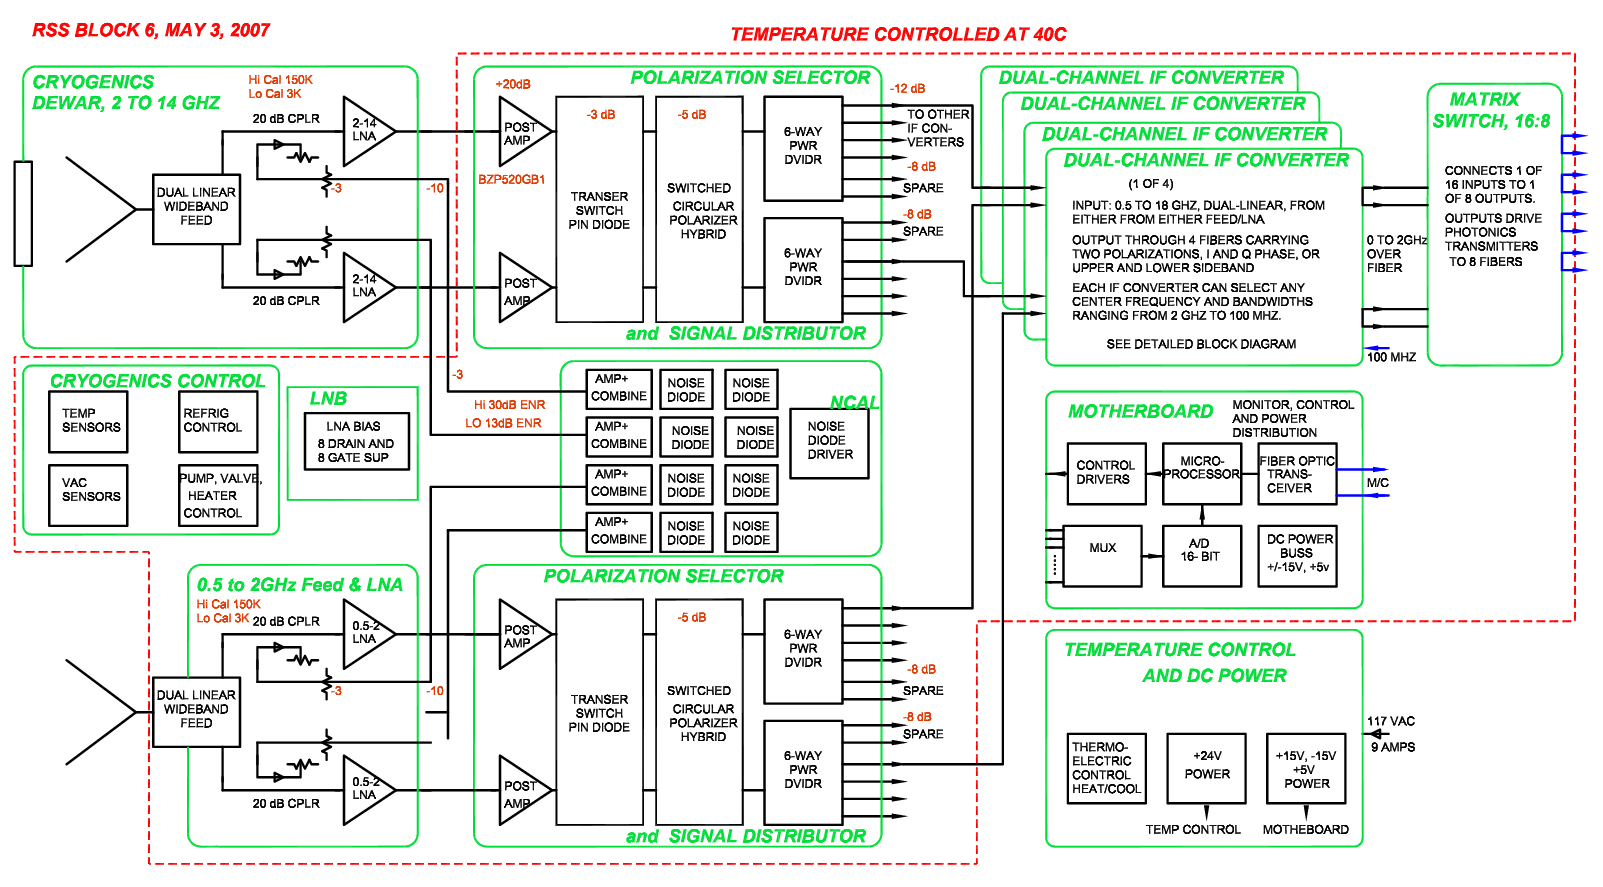
\includegraphics[width=\textwidth]{Block6A_3May07-r.png}
        \caption{\label{fig:rx-overview}Schematic diagram of the
            receiver.}
    \end{center}
\end{figure}
Figure~\ref{fig:rx-dc} shows an overall schematic of a DSS-28 receiver down-converter.
\begin{figure}[h!tb]
    \begin{center}
        % trim arguments: left bottom right top
        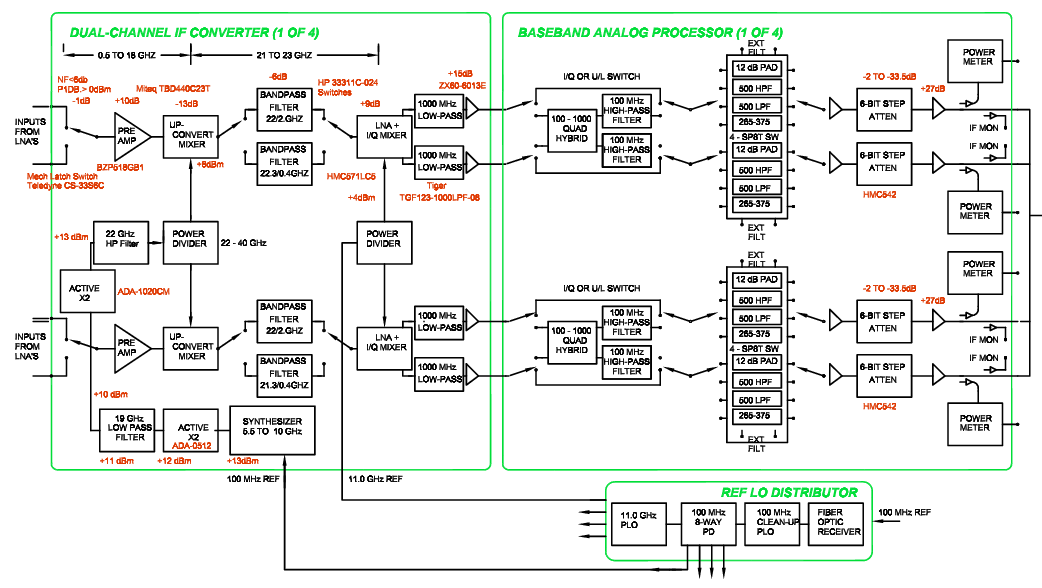
\includegraphics[width=\textwidth]{Block6B_3May07-r.png}
        \caption{\label{fig:rx-dc}Schematic diagram of a down-converter.}
    \end{center}
\end{figure}

\begin{thebibliography}{widestlabel}
   \bibitem[Kuiper and Shaff (2019)]{kuiper:2019}
   Kuiper, T.B.H., and Shaff, D. ``General Purpose Radio Telescope Monitor and
   Control System'', in preparation, 2019.
\end{thebibliography}
\end{document}
